\documentclass[10pt]{article}

\usepackage[utf8]{inputenc}
\usepackage{amssymb}
\usepackage{enumitem}
\usepackage{longtable}
\usepackage{nopageno}
\usepackage{float}
\usepackage{graphicx}
\graphicspath{{./images/}}

\usepackage{rotating}
\def\rot{\rotatebox}

\usepackage{url}
\usepackage{hyperref}
\hypersetup{colorlinks=true, linkcolor=black, filecolor=magenta, urlcolor=blue,
    citecolor=black}

\usepackage[normalem]{ulem}
\useunder{\uline}{\ul}{}
\usepackage{multirow}

\usepackage{geometry}
\geometry{
 a4paper,
 total={170mm,257mm},
 left=10mm,
 right=10mm,
 top=10mm,
 bottom=10mm,
}


\begin{document}


\begin{center}
    \Huge\textbf{CS261 Coursework Design Document}\\
    \vspace{2mm}
    \large{\textit{\textbf{Group 17:} Ben Lewis, Dan Risk, Edmund Goodman,
    Jay Re Ng, John-Loong Gao, Rahul Vanmali, Tomás Chapmann Fromm}}
\end{center}


\section{Introduction}
% \vspace{-6mm}\section{Introduction}\vspace{-2mm}
Deutsche Bank requires a system prototype to support the mentoring process for
employees. The principal purpose of this document is to broadly record the
process documentation and design choices for said system prototype. For process
documentation, this document will detail development methodologies in addition
to workflow and project organisation. Design choices include a prototype user
interface design and technical diagrams demonstrating user interactions between
multiple users and the system. Furthermore, our testing strategy and technical
descriptions such as choice of technologies used and system architecture will be
covered in depth to illustrate more full idea of the final product.

\section{Process documentation and planning}
\subsection{Development methodology}
We opted for an agile development methodology based on the Scrum model. The
development timeline will be broken down into a large initial planning phase and
a series of week-long sprints. We will have multiple meetings each sprint cycle
to assess progress (sprint review) and adapt the plan if required.

An agile methodology is optimal for a short timeframe as it allows rapid product
development with concurrent implementation and testing so we can make effective
use of the time available. It also allows for more flexibility if we face
unexpected delays during development, which is likely with an inexperienced
team. Producing a thorough plan before beginning the agile development process
is suitable since deliverable deadlines are fixed, so ensuring work is completed
on time is critical. Additionally, contact with the client is limited so
requirements are unlikely to change and the project will not deviate much from
the initial plan.

\subsection{Project organisation and communication}
We decided on a flat team hierarchy since we have similar levels of software
development experience, self-managed but with well defined responsibilities. To
communicate between meetings, we decided to use Discord, as it is already a
popular choice within the team and is easy to learn for new users. It offers
both text and voice chat as well as a number of features such as GitHub
integration, so we are notified via Discord when on changes, for example when
pull requests are made.

Discord can be used for online meetings however we aim to convene in-person at
least twice a week, as this enables us to share ideas much more easily and
maintain focus during meetings. At these meetings we can compare progress on the
system with our plan, and assign tasks based on documentation or what tasks need
doing in order to stay on schedule. We will use Trello to assist in the task
management process, as it provides a visual representation of current project
progress.

\subsection{Project schedule}
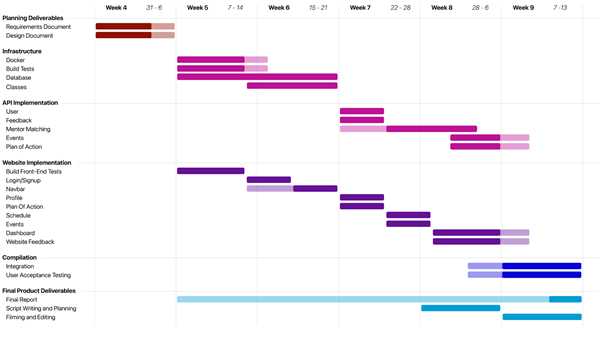
\includegraphics{Timetable}
\\
The timeline outlines which features of the system will be implemented each
week, divided according to the team which is working on them, with final product
documentation separated as this is a collaborative effort by the whole team. As
we are following a Scrum methodology, task order may be adjusted weekly so that
the project remains on track, so which features are completed in each week will
most likely change. It also acts as a reminder that the final report should be
completed, when time is available, concurrently with the project itself, so it
doesn’t need to be written in its entirety in the few days before submission.
\subsection{Risk management}

% \begin{table}[]
\begin{longtable}{|p{0.15\linewidth}|p{0.15\linewidth}|p{0.1\linewidth}|p{0.08\linewidth}|p{0.15\linewidth}|p{0.15\linewidth}|p{0.08\linewidth}|}
\hline \rot{45}{\textbf{Risk}} & \rot{45}{\textbf{Impact}} & \rot{45}{\textbf{Likelihood}} & \rot{45}{\textbf{Severity}} & \rot{45}{\textbf{Mitigation}} & \rot{45}{\textbf{Contingency}} & \rot{45}{\textbf{Residual}} \\ \hline\hline
    Team members unable to work & Smaller team until the member can resume work                     & 2 & 7 & Team members take precautions                                 & Reduce scope and reallocate work across team  & 2 \\ \hline
    Task longer than expected   & Project delayed until task completed                              & 5 & 4 & Allocate buffer time to allow overrunning tasks               & Re-assign team members to load balance        & 4 \\ \hline
    Poor code quality           & System fails testing or linting procedures                        & 5 & 4 & Code review and automated testing through CI/CD               & Re-assign team memebrs to fix pair program    & 3 \\ \hline
    Requirements change         & Design and existing code must be changed                          & 3 & 8 & Use an agile methodology to facilitate requirements change    & Update project plan and proceed with new one  & 3 \\ \hline
    Code lost                   & Code must be re-written                                           & 1 & 7 & Use `git` as version control, and remote backup to GitHub     & Restore code from local or remote backups     & 1 \\ \hline
    Problems with dependencies  & Component of project fails external library or technology         & 2 & 4 & Choose technologies and dependencies carefully                & Find replacement library or technology        & 2 \\ \hline
    Scope creep                 & Addition of unnecessary features causing growth of project scale  & 7 & 4 & Include extra features in project timeline, and stick to it   & Drop lowest priority features                 & 5 \\ \hline
\end{longtable}
% \caption{}
% \label{tab:my-table}
% \end{table}

\section{Technical description}

\subsection{Scope}
Our system must satisfy a complex specification, so its development must be
carefully planned and executed. However, the goal is to create a prototype, not
a finished product. As such, various aspects which might be required for a
system going into production are not needed within a prototype.

One example of this is limitations on the scalability, for example the number of
concurrent users. It is much more important that key features are implemented
than being able to support dynamically changing high numbers of concurrent
users, as the prototype will likely only be tested by a few users at any time.
However, this does not mean that the prototype should not be designed without a
good basis for facilitating scalability later as the system moves through its
lifecycle. Another example of this is the use of Deutsche Bank branding, which
is explicitly not to be used, although it would be incorporated in the
production system. Instead, a generic and simple theme should be used in the
prototype, which could then be later replaced with the correct branding.

\subsection{System attributes}
This section will communicate the different qualities needed by software, what
is within our scope, how we have addressed them, and what we are not doing for
this prototype.\\ The end goal of the software engineering lifecycle is to end
with satisfied customers. As such, it is crucial that usability of the software
is given important consideration. Our goal is to ensure that the website is
intuitive to use, has little ambiguity and can be learnt ideally without
assistance even for non-technical users. There will be a wide coverage of
acceptance testing carried out to ensure this is achieved. Along with this, our
prototype aims, if possible, to make our system accessible to people with
disabilities with features such as enlarging text and higher contrast colours.
\\Compatibility and portability are important points to consider since we want to
make our system as portable as it needs to be, and compatible with systems used
by most of our users. Being a web app, makes it portable since every user will
have some access to a device able to run a browser. Extreme cases such as legacy
browsers will not be prioritised since it is unlikely to be used. The prototype
will not include desktop and mobile applications since it is out of the scope
and not needed with a web app, this early in the mentoring system. \\Security is a
relevant quality to consider, especially since we do not want to create issues
for any relevant parties involved. Complete and effective considerations to
security for most areas of vulnerability is out of scope for a prototype
implementing its core functionalities. Important security details such as
account access protection through salted/hashed stored passwords are to be
implemented. Data will only be accessed through the REST API, allowing us to
ensure only required data is sent, and adds a layer of security since our
database is not directly interacted with. Allows us to also validate any user
information before storing it in the database.

\subsection{Technologies used}

% NEED TO UPDATE THIS TO USE TABLE
A fundamental decision in the project is deciding which technologies should be
used to compose the so-called “tech stack”. Since this is such an important set
of decisions, we carefully considered a number of options with respect to a set
of criteria which assess the quality of a component technology choice. These
criteria include:\\ 
\begin{itemize}
    \item Suitability, how well does the technology match the problem
our system solves? 
    \item Documentation and popularity, does the choice have strong
documentation and an active community likely to have already answered problems
we may encounter? 
    \item Consistency, how well the choice meshes with the other
component technologies? 
    \item Performance, will the technology run sufficiently fast,
and can it be scaled later needing to switch to something else more performant?
    \item Experience, how much prior knowledge does our team have of the technology? 
\end{itemize}

We decided to implement the project as a web application, as opposed to a mobile or
desktop only one. This is because it is generic and can be accessed by almost
all users, as essentially every modern device has a web browser. However, this
design choice must later be taken into consideration when ensuring the UI is
suitable for mobile. This choice was made as the system must be widely
accessible by users with many different types of devices, and a web application
was the only suitable choice for this.

We chose Django for our backend framework, which runs on top of Python. This is
suitable for our system as it facilitates fast development, which is required to
finish our prototype in the very short turnaround of around five weeks, with
very short code sprints, and it inherently supports our non-functional
requirements of security and scalability. Furthermore, it has robust
documentation and is widely used with an active community. Additionally, Python
is so ubiquitous that it can interface consistently with almost any other
technology choice, for example persistent data storage and sentiment analysis.
Finally, our team has a lot of experience with Python development, and
additionally testing techniques for Python, mitigating learning curves and
ensuring bug-free code.

Since we are making a web application, we will use HTML/CSS/JS. We decided to
use the Vue.JS framework for the frontend JS, as it facilitates writing
responsive websites, but has a much less steep learning curve than other
frameworks such as React, and is known to integrate well with Django, the
backend framework we propose using. Furthermore, we are going to use bootstrap
as the CSS framework as it allows us to quickly develop a professional looking
website with little hassle by providing building block CSS classes. 

We chose PostgreSQL to store our persistent data in the form of a relational
database. This is because the type of data recorded by the system is well suited
to storage in a relational schema. For example, storing a set of users, each of
whom have various properties and relationships with other users is a very good
match for this model. Furthermore, postgresql has very good documentation in
comparison to other relational databases, and it meshes well into our tech stack
as django and postgresql are commonly used in tandem. Finally, all of our team
has experience with it due to the CS258 databases module.

We chose the python library NLTK (natural language toolkit) to implement our
sentiment analysis. This is because it is compatible with the rest of the
backend framework, which is already written in python, and it is the most
popular and widely used library within its field.

We will use JSON for the REST API, as it is incredibly ubiquitous, and links
easily into most web frameworks, as it is a subset of javascript. Additionally,
both our backend and frontend team members have experience with it, which is
crucial as it will form the link between the two sides of the technology stack,

We chose docker for our containerisation. This supports all of the rest of the
tech stack, and allows “lift-and-shift”, which is a very useful property for
prototype systems. Additionally, it is by far the most widely used choice for
containerisation, and has good documentation. Finally, none of our team has
experience with any form of containerisation, so choices cannot be compared by
this metric.

We chose git with GitHub for our version control. This is because it is the
industry standard for version control, every member of our team had at least
rudimentary experience with it from CS133, and some members of our team had
experience with advanced features for CI/CD such as GitHub Actions.

\subsection{System architecture}
Our system architecture follows the MVC (Model View Controller) architecture
which is a well-known model to be successful in creating a system that presents
data obtained through a controller that interacts with the database. This is
reflected in the docker containerisation figure with our website being the view,
the Django system being the controller, and Postgresql as the model. Being
modularised to 3 separate components, allows easy distribution of development,
with each focusing on a subset of skill sets. One downfall is that the system is
tightly connected in that if one system fails, the rest falls… (include REST API
also easy reference).\\
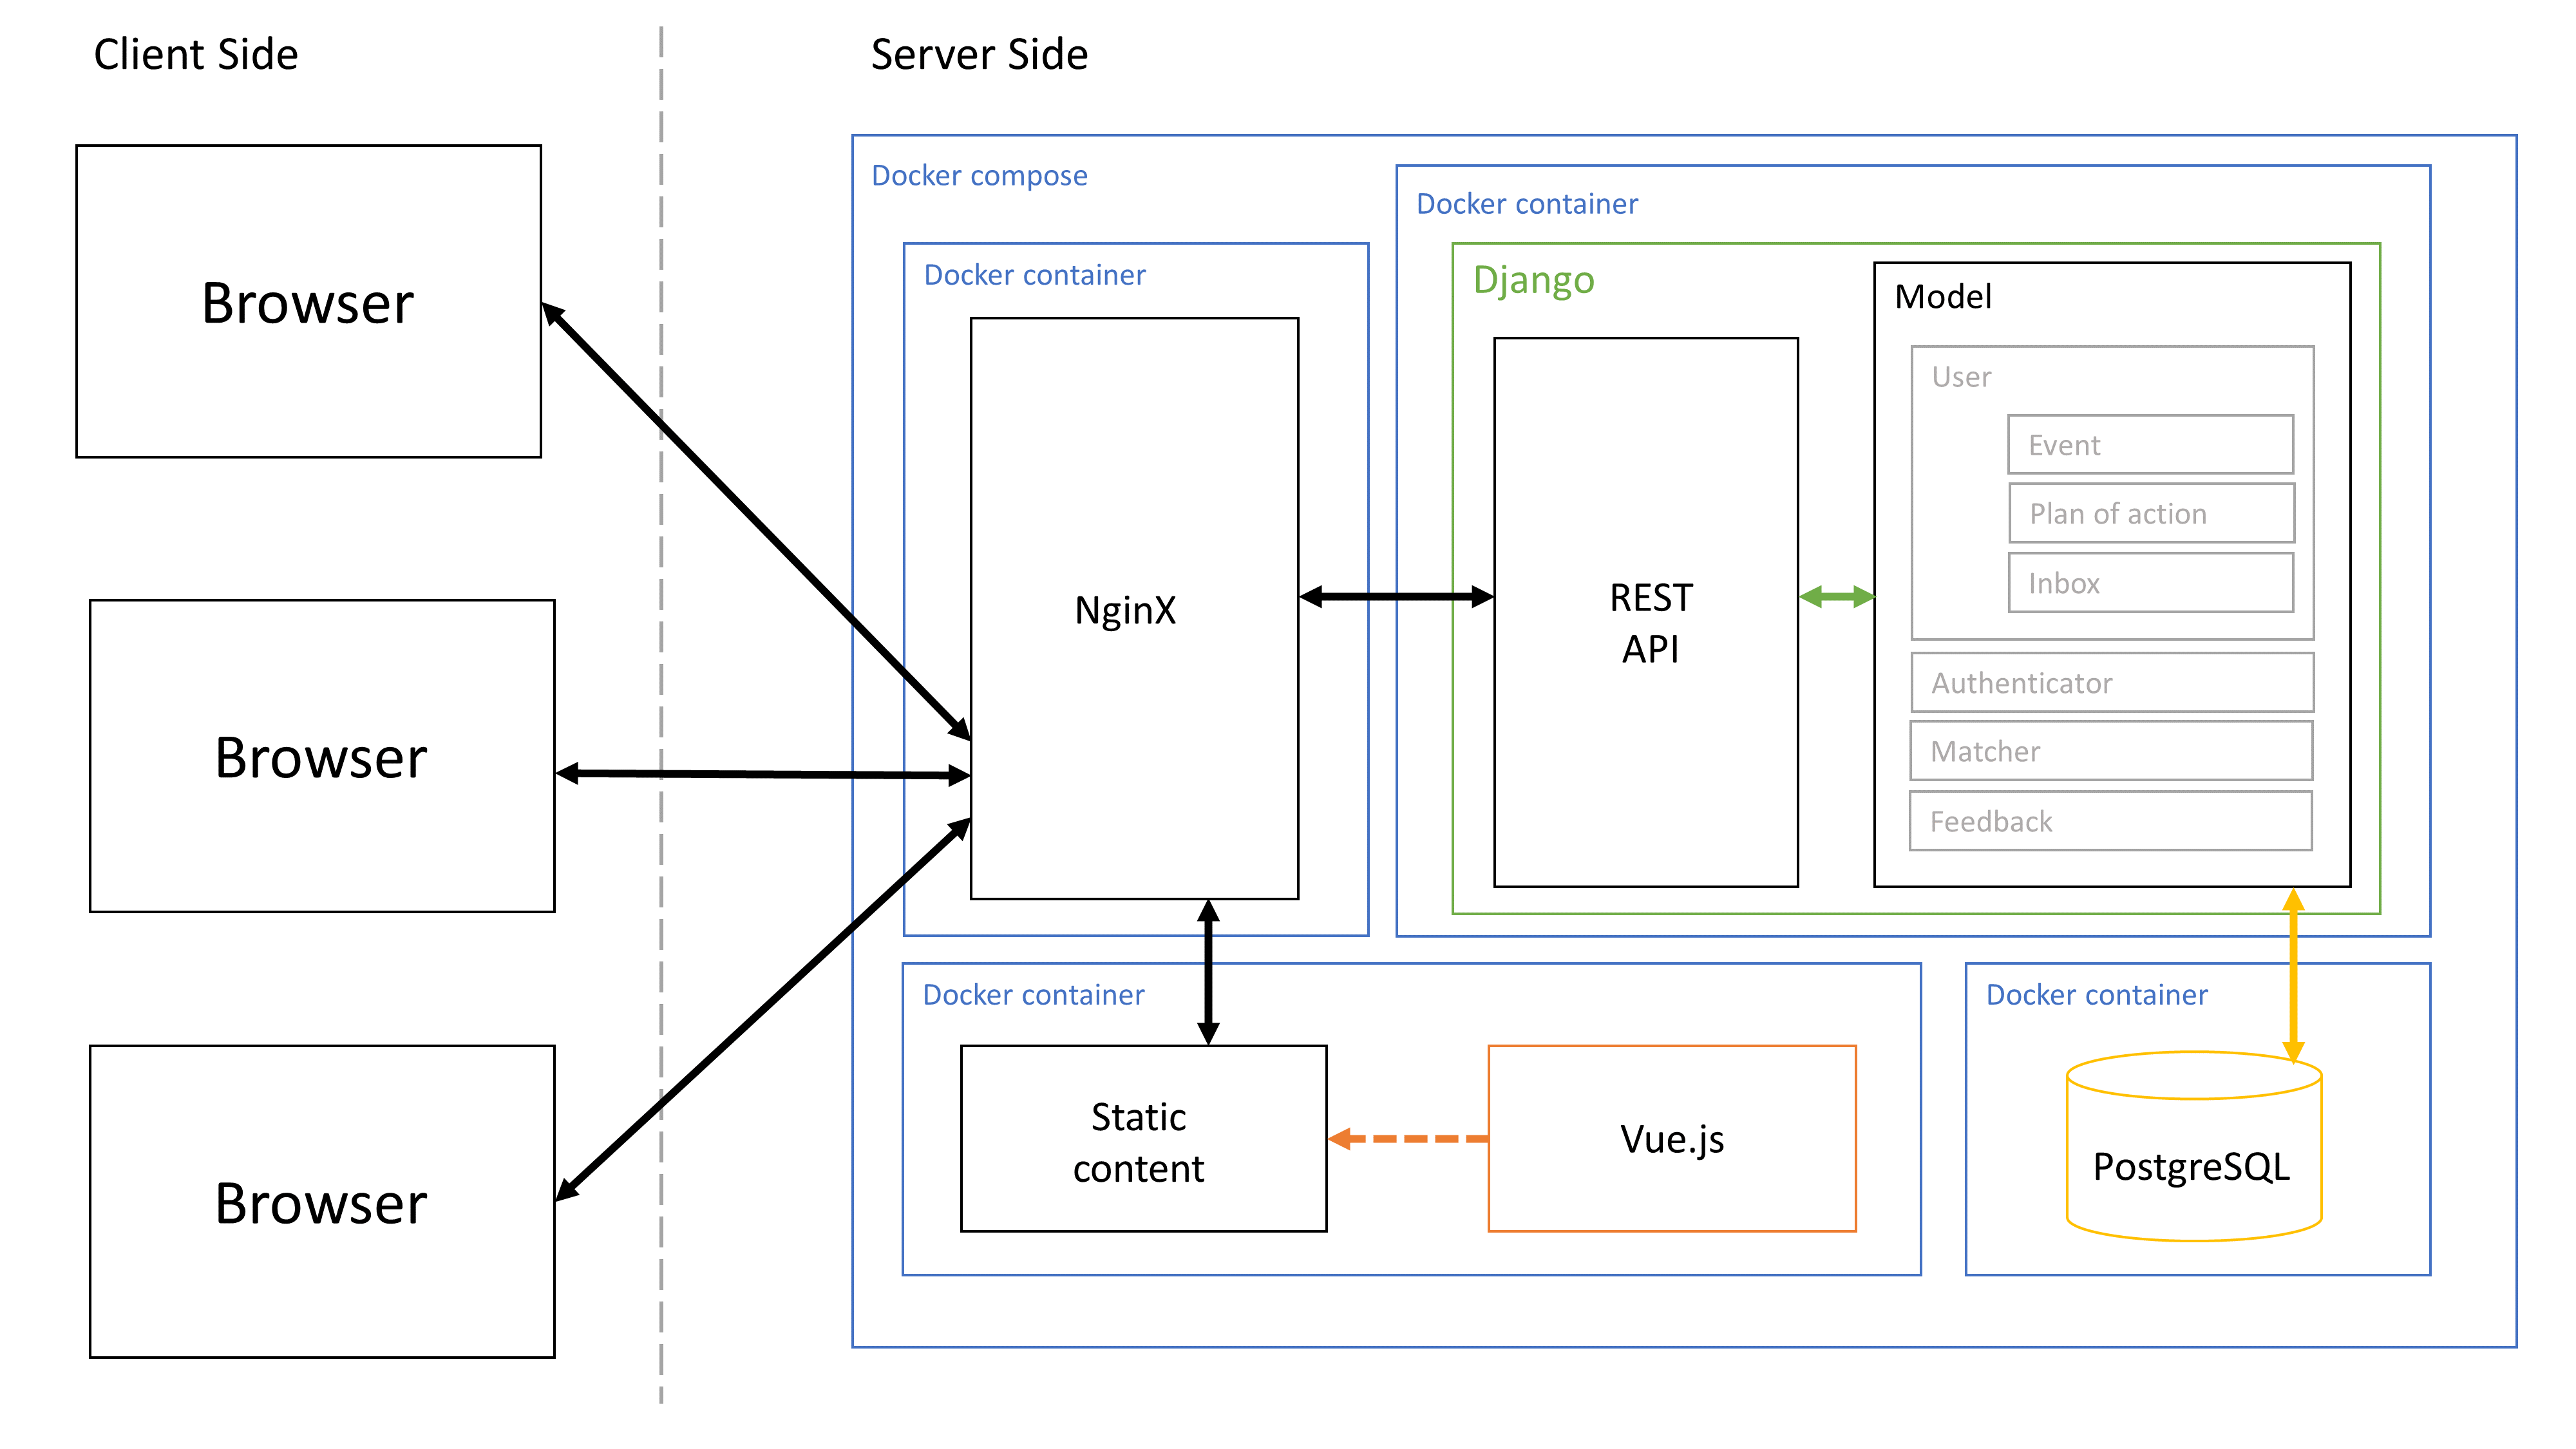
\includegraphics{architecture}

\subsubsection{Database Design}
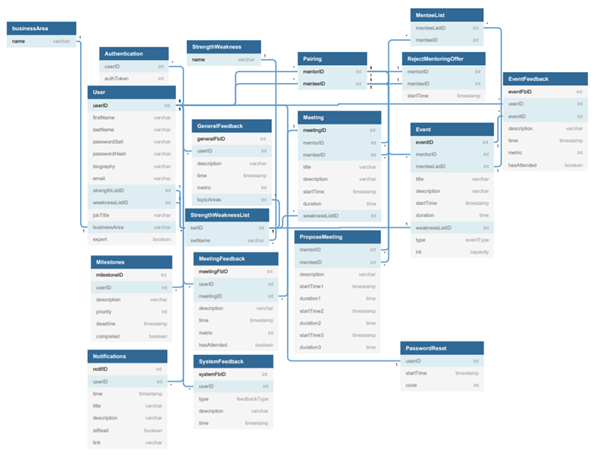
\includegraphics{DB}

\subsubsection{Object Structure}
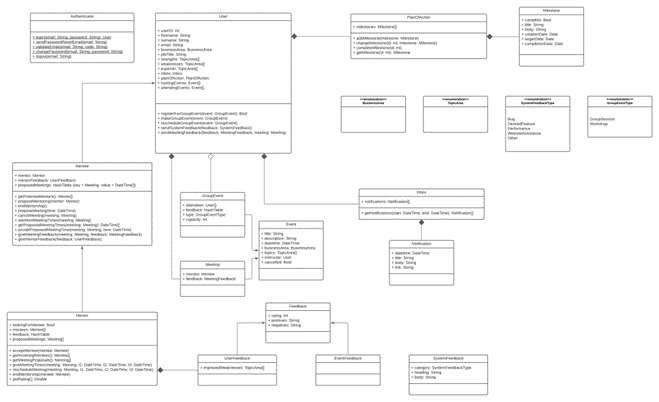
\includegraphics[scale=0.32]{Objects}

\subsubsection{API design}
% Edmund do it, long table

\section{UI/UX design}

\subsection{Page Hierarchy}
The page hierarchy below displays the sites that our webpage comprises of. Here
is a brief outline of what each page will consist of: 
\begin{itemize}
    \item Login Screen: The landing page of the website that allows the user to
    login to go to the dashboard or the sign up page to create an account. 
    \item Sign Up: Allows the user to create an account. 
    \item Dashboard: The central hub for the user where all pages can be
    accessed from and displays useful information that may be useful (look at
    page designs for more detail). 
    \item Profile: This page has 3 purposes: resetting the users password,
    seeing the users data and modifying the users data. 
    \item Plans of Action: Displays the users plan of action and their mentees
    plans of actions too if they have any. 
    \item Individual POA: If the user clicks on a POA, then they come to this
    page where the POA can be viewed and modified. 
    \item Schedule: Shows the users schedule, allows them to request meetings
    and has a list of feedback and meeting requests that the user should respond
    to. 
    \item Group Events: Allows the user to search for workshops and group
    sessions within the system that they can attend.
    \item Individual Event: A page that details an event (meeting or group
    event) and allows the owner of an event to modify or delete the event.
\end{itemize}

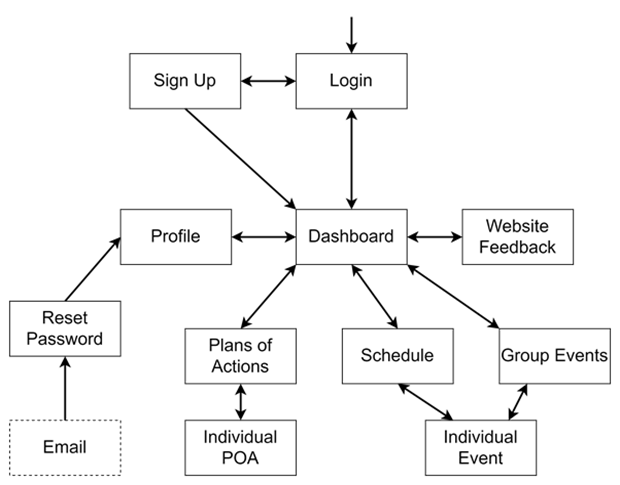
\includegraphics[scale=0.25]{Hierarchy}

\subsection{User-system interaction}
The specification was also very vague about how to match up mentors and mentees,
therefore this diagram clarifies all the ambiguities around this.
\begin{itemize}
    \item The user can only have 1 mentor at a time
    \item The system can give the user a list of potential other users who are currently looking for mentees
    \item The user then picks one of these users and a mentor mentee request is sent to the potential mentor
    \item If the potential mentor accepts, then a relationship is formed
    \item Otherwise, the mentee needs to choose another mentor from the list
\end{itemize}
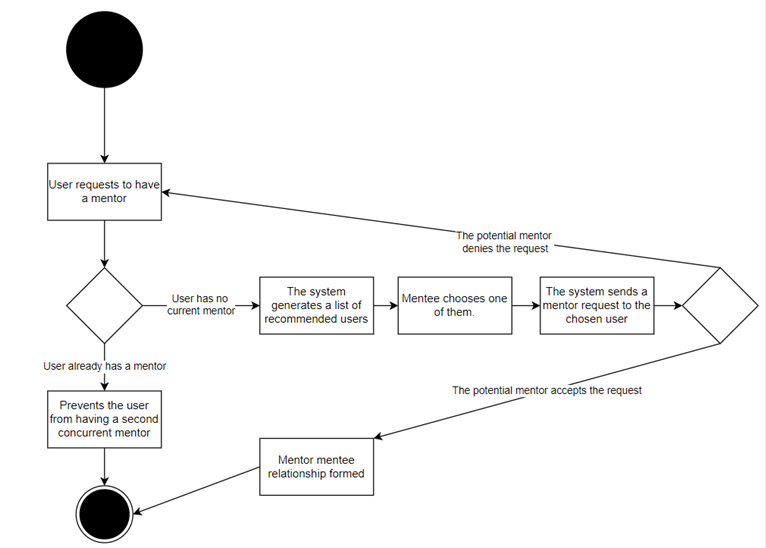
\includegraphics[scale=0.7]{MentorMentee}

The diagram below displays what functions the Schedule page has. This handles a
lot of ambiguities around how the meeting and feedback system will work within
our system. The important points from this diagram is that:
\begin{itemize}
    \item Mentee’s can cancel meetings, but mentors can only reschedule
    \item Mentee’s can request a meeting, but mentors cannot not
    \item For a meeting to be officially approved, both parties need to agree on the time and date otherwise they go into this loop of suggesting times to each other
    \item The user will be prompted on the schedule page to give feedback to recent events they have gone to
\end{itemize}
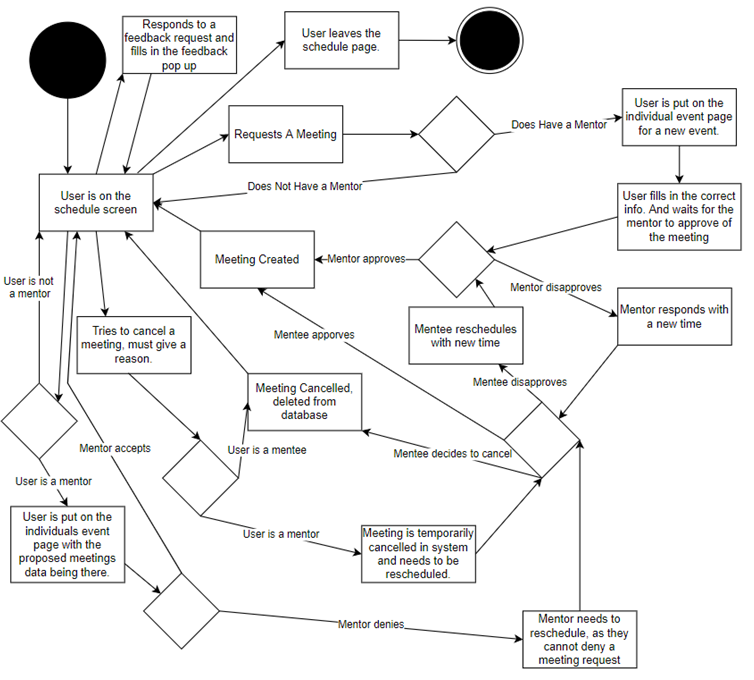
\includegraphics[scale=0.7]{Meeting}

\subsection{Page Design}
The dashboard is the central page for users that displays all the useful
information for the user, such as their upcoming meetings, their current plan of
action and allows them to get a new mentee or mentor. The navigation bar at the
top of the page will be on most of the pages and will allow the user to access
all the other pages of the website as well as their notifications. The
notifications inform the user about any recent events that they may be
interested in such as giving feedback about a recent event or a mentee/mentor
meeting coming up. The drop down button next to the notification bell will link
to the user’s profile page, the website feedback form and a sign out button.
\\
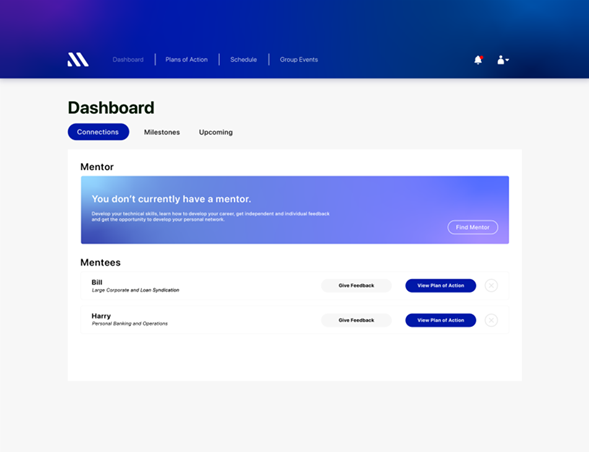
\includegraphics[scale=0.3]{Dashboard}
\\
The schedule page will have the users calender and all the requests the user has
(meeting and feedback). This user is not a mentee so the request meeting button
at the bottom is currently missing, but if the user was a mentee then there
would be a request meeting button at the bottom. Additionally, clicking on a
meeting will take the user to the individual event page for the meeting which
will have the feedback log for the meeting.
\\
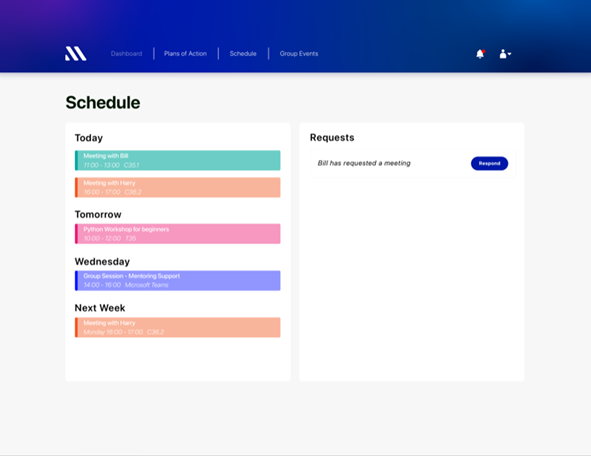
\includegraphics[scale=0.3]{Schedule}

\section{Testing}
\subsection{Test cases}
% Need to use a long table, Edmund
\subsection{Unit and integration testing}
Tests will form an integral part of our development cycle, as we plan to follow
the agile test driven development ideologies. We will implement this by creating
unit tests for all of the above test cases, allowing us to ensure all the
required properties of the system are met. These can then be run throughout the
development process. All of the tests will be automatically run on a pull
request to the GitHub repository, and must pass in order for the code to be
merged into the main branch, to ensure its validity. This is an implementation
of “continuous integration” from CI/CD, and will be implemented using GitHub
actions.

There are many tools for unit testing which can be used. Since we are using a
python backend framework, we will use PyTest for unit tests on the backend code,
along with codecov to assess the coverage of the tests, and pylint to ensure
that stylistic code is being written. Since we are using a javascript frontend
framework, we will use Jest for unit tests on the frontend code and UI, along
with ESLint to check that the Javascript is correct. Finally, we will use
Postman to test that the API serves the correct data. There are relatively few
tools for integration testing, and it will likely mostly have to be done by
hand. We will use the Puppeteer tool to automate this task as far as possible.
The combination of all of these tools allows us to create a testing suite which
will fully cover our system.


\bibliographystyle{ieeetr}
\bibliography{designDocument.bib}


\end{document}
